\documentclass[12pt,a4paper]{article}
\usepackage{geometry}

% Page margin layout
\geometry{left=2.3cm,right=2cm,top=2.5cm,bottom=2.0cm}

\usepackage{graphics}
\usepackage{graphicx}
\usepackage{subfigure}
\usepackage{epsfig}
\usepackage{float}
\usepackage{mfirstuc}
\usepackage{hyperref}
\usepackage{amsmath}

\usepackage{booktabs}
\usepackage{threeparttable}
\usepackage{longtable}
\usepackage[ruled,linesnumbered]{algorithm2e}
\usepackage{listings}

% cite package, to clean up citations in the main text. Do not remove.
\usepackage{cite}

\usepackage{color,xcolor}

%% The amssymb package provides various useful mathematical symbols
\usepackage{amssymb}
%% The amsthm package provides extended theorem environments
\usepackage{amsthm}
\usepackage{amsfonts}
\usepackage{enumerate}
\usepackage{enumitem}
\usepackage{listings}

\usepackage{indentfirst}
\setlength{\parindent}{2em} % Make two letter space in the first paragraph
\usepackage{setspace}
\linespread{1.5} % Line spacing setting

\setlength{\parskip}{0.5em} % Paragraph spacing setting

%%%%%%%%%%%%%
\newcommand{\TeamNumber}{2208487}  % Fill your team number here
\newcommand{\Problem}{C}  % Replace your team chosen problem here
\newcommand{\PaperTitle}{To Harvest More: Best Trading Strategies on Gold and Bitcoins}  % Change your paper title here
%%%%%%%%%%%%%

\newcommand{\Predictor}{ARIMA }
\newcommand{\Decision}{Markowitz mean-variance model }
\newcommand{\DecisionAssessment}{Sharp ratio}

%% Page header and footer setting
\usepackage{fancyhdr}
\usepackage{lastpage}
\pagestyle{fancy}
\fancyhf{}
\fancyhead[L]{\texttt{Team \#  \TeamNumber }}
\fancyhead[R]{\texttt{Page {\thepage} of \pageref{LastPage}}}



\begin{document}

%%%%%%%%%%%%%%%%%%%%%%%%%%%%%%%%%%%%%%%%%%%%
\makeatletter % change default title style
\renewcommand*\maketitle{%
    \begin{center} 
        \bfseries  % title 
        {\LARGE \@title \par}  % LARGE typesetting
        \vskip 1em  %  margin 1em
        {\global\let\author\@empty}  % no author information
        {\global\let\date\@empty}  % no date
        \thispagestyle{empty}   %  empty page style
    \end{center}%
  \setcounter{footnote}{0}%
}
\makeatother
%%%%%%%%%%%%%%%%%%%%%%%%%%%%%%%%%%%%%%%%%%%%


%%%%%%%%%%%%%%%%%
% Summary sheet
\begin{table}[h]
\renewcommand{\arraystretch}{1.2}
\label{Summary}
\begin{center}
\resizebox{\textwidth}{!}
{\large
\begin{tabular}{c c c c c c c}
{\,} & \textbf{Problem Chosen} & {\qquad \quad} & \textbf{2022} & {\qquad \quad} & \textbf{Team Control Number} & {\,}\\
{} & \raisebox{-2ex}[0cm][0cm]{\LARGE{\textbf{\textcolor{red}{\Problem}}}} & {} & \textbf{MCM/ICM} & {} & \raisebox{-2ex}[0cm][0cm]{\LARGE{\textbf{\textcolor{red}{\TeamNumber}}}} & {}\\
{} & {} & {} & \textbf{Summary Sheet} & {} & {} & {}\\
\bottomrule
\end{tabular}}
\end{center}
\end{table}
\vskip -1.5em
%%


\begin{spacing}{1.2}   % summary line spacing setting


% Enter your summary here replacing the (red) text
% Replace the text from here ...

Traders buy and sell volatile assets to maximize their income. Recently, with the growing interest of the public in cryptocurrencies, gold and bitcoin become a feasible combo. Our team is requested to determine the trading strategies for a trader which uses only the past daily prices. 

As for problem 1, First we plot the price data and found that they show non-stationarity in the sense of mean. We therefore utilize \Predictor to predict the prices of gold and bitcoin. The predictor shows good capability to accurately predict the price of future.

To find the best timing to sell and buy the two assets, we first rate them with the percentage change, based on predicted value. Then we accomplish position management with Markowitz model. The choice we made yields good income.

As for problem 2, we

As for problem 3, we

Finally


\textbf{Key words:} 

\end{spacing}

\thispagestyle{empty}


%%%%%%%%%%%%%%%%%
\newpage

\title{
\Large{\textcolor{black}{\PaperTitle}}
}




\maketitle



%%%%%%%%%%%%%%%%%
% Table of Contents
\tableofcontents
\setcounter{tocdepth}{2}

%%%%%%%%%%%%%%%%%
\newpage
\setcounter{page}{1}

%% main text

\begin{spacing}{1.2} 



%%%%%%%%%%%%%%%%%
\section{Introduction}
\label{Problem_Statement}

\subsection{Problem Background}
With the popularity of cryptocurrencies and the simplification of trading methods, more of the population become market traders. Some of them expect to outperform inflation, while others want to create wealth. By buying and selling volatile assets frequently, market traders pursue a goal to maximize their total return. Gold and bitcoins enjoy great popularity these days for their complementary characteristics in risk and value. Gold is stable in price and has lower risk while the value of bitcoins varies greatly and thus has a higher risk, as is shown in Figure \ref{figure:prices2in1}.

\begin{figure}[H]
	\centering{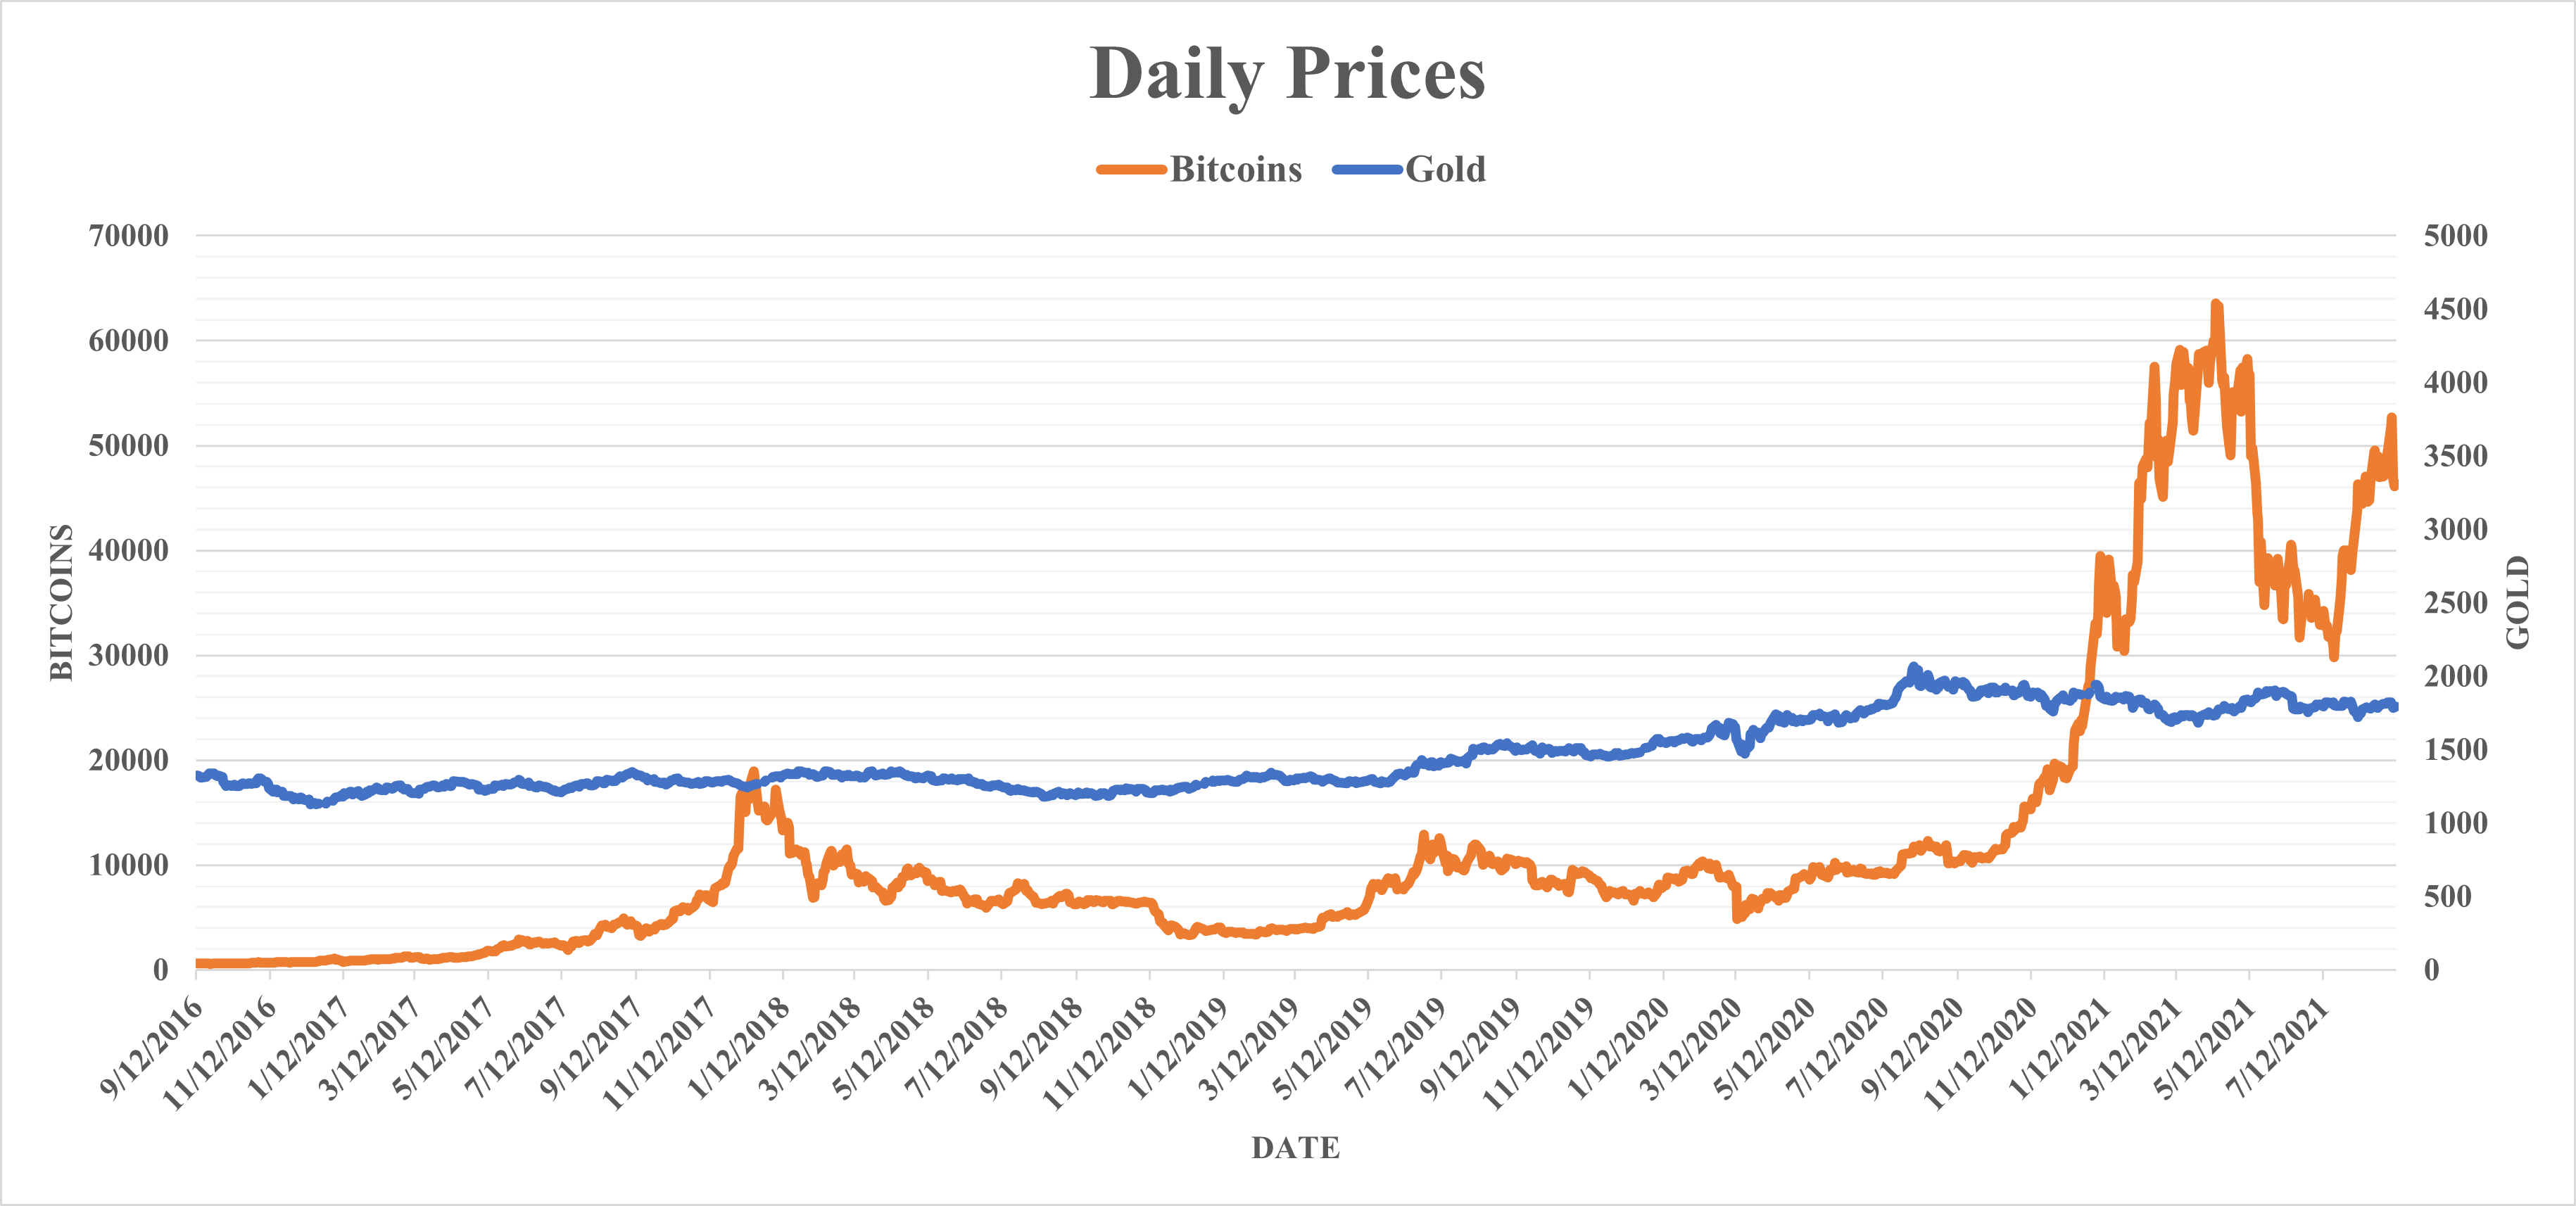
\includegraphics[width=17.0cm]{figures/prices_2in1.png}}
	\caption{Gold and bitcoin daily prices, in U.S. dollars per troy ounce and U.S. dollars per bitcoin. \textbf{Source:} London Bullion Market 
		Association, 9/11/2021 and NASDAQ, 9/11/2021 }
	\label{figure:prices2in1}
\end{figure}

 Regarding trading rules, Gold is only traded on days the market is open while bitcoins are traded every day. Commissions are charged to make each transaction. For market traders to achieve their goals, they need to build a model to determine the strategies to manage their portfolios well.

\subsection{Restatement of the Problem}

\begin{itemize}
	\item Develop a model that gives the best daily trading strategy based only on price data up 
	to that day, and calculate how much the initial \$1000 investment is worth on 9/10/2021 using the 
	model and strategy.
	
	\item Present evidence that your model provides the best strategy.
	
	\item Determine how sensitive the strategy is to transaction costs and analyze how the costs
	affect the strategy and results.
	
\end{itemize}

\subsection{Our Approach}

\begin{enumerate}
	\item \textbf{To predict the prices of bitcoin and gold and make decision, we use \textit{\Predictor} (Autoregressive integrated moving average).}
	To predict future prices with existing data is a difficult problem because too many factors may influence the prices. The international situation, national policies, and even social media can have a considerable impact on the prices. Moreover, the data shows non-stationarity. To take as many factors as possible and predict accurately according to their inner laws, we adopt this approach to predict the prices, which is proved to give satisfying results.
	
	\item \textbf{To make decision on trading, we adopt \textit{\Decision} and \textit{\DecisionAssessment}. }
\end{enumerate}

%%%%%%%%%%%%%%%%%
\section{Assumptions and Justifications}
\label{Assumptions_Justifications}

\subsection{Assumptions}
To simplify the problem stated above, we make following assumptions, each of which is justified properly: 
\begin{enumerate}
	
	\item \textbf{The trader does not have a bias towards a lower risk.} The two given assests, gold and bitcoin, differs a lot in risk. To simplify the problem, we assume that the trader will not prefer lower risk than higher and only cares about higher income.
	
	\item \textbf{The trader will have \$1000 in the beginning, and the transaction commissions for gold and bitcoin are $\alpha_{gold}=1\%$ and $\alpha_{bitcoin}=2\%$, respectively.}


	\item \textbf{The market trader sells all of the gold and bitcoins by the end of the five-year trading period, i.e. on 9/10/2021.} Generally, investors cares about funding liquidity. Among cash, gold and bitcoins, only cash can circulate unhindered in the market. So we make this assumption and thus measure the outcome in cash.
	
\end{enumerate}


\subsection{Symbols and Definitions}



\subsection{Symbols and Definitions}





%%%%%%%%%%%%%%%%%


\section{Data Preprocessing}
\label{DataPreprocessing}


\subsection{Metric Calculating}

\subsubsection{Average Change}

Using the trained predictor, we calculate the average of change in the period of 5,10,15,20,and 25 days.

The change each day is defined as

$$
Percentage \ change = PC = \frac{New \ price-Old \ price}{Old \ price} \times 100\%
$$


The result for the given data is in the \nameref{sec:AppendixFT}. Figure \ref{figure:bitcoin_ac} and Figure \ref{figure:gold_ac} shows the average change we calculated for bitcoin and gold, respectively.


\subsubsection{Bias}

Bias measures how much the closing price shifts from the average price.

The formula to calculate the Bias in a $n$ day period is

$$
Bias = \frac{Closing \ price}{The \ mean \ price \ of \ n \ days} - 1
$$

Bias can help to track the market for the raise and fall of the price, which help us to decide whether and when to sell or buy.

\subsubsection{Moving Averages (MA)}

An $n$ day's MA is the average of the price today and the previous $n-1$ days. Plotting all the MAs in a chart, it can reveal the trend of the price of the given period. Combined with current price, it helps us to find the favorable timing to increase our outcome

\section{Mathematical Modeling}
\label{MathModels}

\subsection{\Predictor Predictor}

\Predictor is widely used for forecasting time series data, which is a generalization of ARMA (autoregressive moving average) model. ARMA requires the mean function of the data to be stationary, because history data of stationary series can be used to predict the future. But time series are not always stationary, so ARIMA take an initial differencing step to eliminate the non-stationarity of the mean function. In this case, we find the first order difference is stationary, so we take first order difference. Figure \ref{figure:flow_chart} shows the procedure we take to build the \Predictor model.

 \begin{figure}[H]
 	\centering{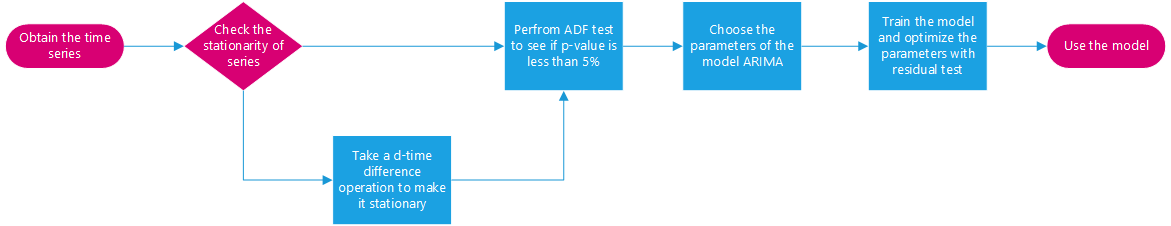
\includegraphics[width=16.0cm]{figures/flow_chart_arima.png}}
 	\caption{Procedure to Build ARIMA Model}
 	\label{figure:flow_chart}
 \end{figure}


To apply the model, we first have to test the stationarity.

\subsubsection{Augmented Dickey-Fuller Test}

An augmented Dickey–Fuller test (ADF) is a kind of hypothesis test. The null hypothesis is 

$$
H_0 \ : \ A \ unit \ root \ is \ present \ in \ a \ time \ series \ sample.
$$

Subject to the $\chi^2$ distribution, we accept it when the observed value of the waviness of the series, $P$, also known as the $p-value$, satisfies

$$
P \ge 0.05
$$

It can test whether the data is stationary or trend-stationary. If the unit root is present in the series, the time-series is non-stationary.

In the raw data, we found

\begin{align*}
	P_{0,bitcoin} &=0.8420802907198858 > 0.05 \\
	P_{0,gold} &=0.9042384812941653 > 0.05 
\end{align*}


So we accept $H_0$. The raw time series is non-stationary.
And in the first-order difference, we found


\begin{align*}
	P_{1,bitcoin}=9.276161468079189e-13 < 0.05 \\
	P_{1,gold}=9.269711421536524e-13 < 0.05
\end{align*}

The first-order difference is stationary, So we plot them in Figure \ref{fig:diff}. 

\begin{figure*}
	\begin{center}
		\subfigure[Gold $1^{st}$ Order Difference]{
			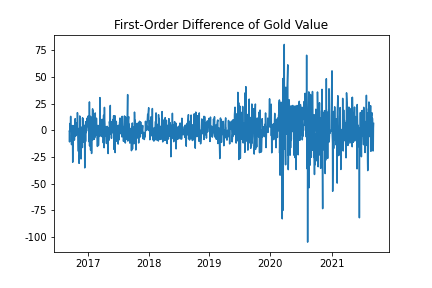
\includegraphics[width=6.0cm]{figures/gold_diff.png}
		}
		\subfigure[Bitcoin $1^{st}$ Order Difference]{
			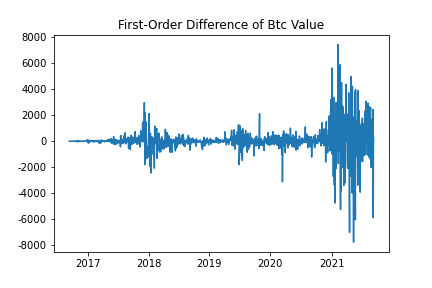
\includegraphics[width=6.0cm]{figures/btc_diff.png}
		}
		\caption{The $1^{st}$ Order Difference}
		\label{fig:diff}
	\end{center}
\end{figure*}

We also can see from the plot that it is stationary. Therefore, we use it for our ARIMA model. The parameter $d$ of $ARIMA(p,d,q)$ is $d=1$.

\subsubsection{Finite Difference}

The difference of a function $y$ is defined as

$$
\Delta^k y_t = \Delta(\Delta^{k-1}y_t)=\Delta^{k-1}y_{t+1}-\Delta^{k-1}y_t=\Sigma_{i=0}^k(-1)^i C_k^iy_{t+k-1} \ (k=1,2,3,\dots)
$$

Specially, the first-order difference, which is commonly used in \Predictor model, is defined as

$$
\Delta y_t = y_{t+1} - y_{t}
$$

Finite difference is useful in processing non-stationary data.

\subsubsection{Choice of Parameters}

To select the best parameters of ARIMA model, we first rely on observation on PACF and ACF plot. And then, if it does not fall in a range that makes sense, we search for possible parameters by grid searching the feasible domain.

\begin{figure*}
	\begin{center}
		\subfigure[Gold ACF Plot]{
			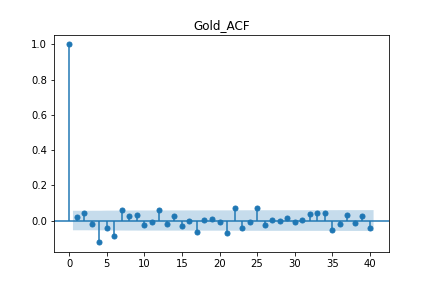
\includegraphics[width=6.0cm]{figures/gold_acf.png}
		}
		\subfigure[Bitcoin ACF Plot]{
			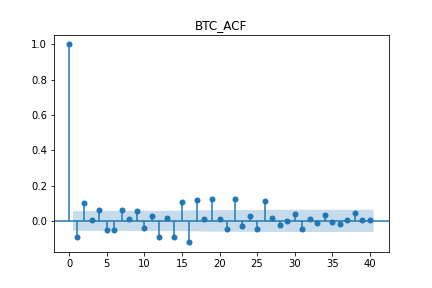
\includegraphics[width=6.0cm]{figures/btc_acf.png}
		}
		\caption{ACF Plot for Gold and Bitcoin}
		\label{fig:acf}
	\end{center}
\end{figure*}

The parameter $p$ of ARIMA(p,d,q) is the number of lag observations in the model, which is also known as the lag order. To assign $p$, ACF plot in Figure \ref{fig:acf} is inspected. We find that $p=4$ is the best choice for both bitcoin and gold.

\begin{figure*}
	\begin{center}
		\subfigure[Gold PACF Plot]{
			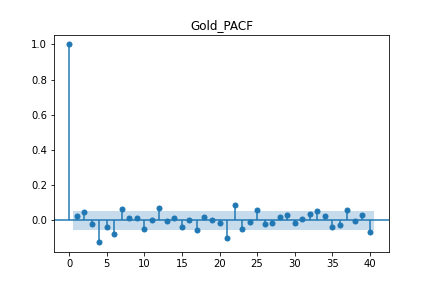
\includegraphics[width=6.0cm]{figures/gold_pacf.png}
		}
		\subfigure[Bitcoin PACF Plot]{
			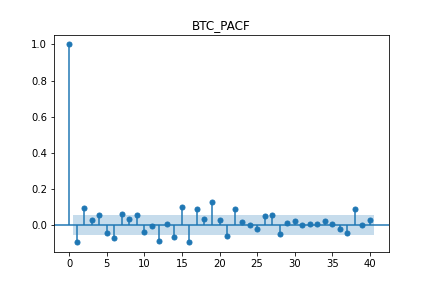
\includegraphics[width=6.0cm]{figures/btc_pacf.png}
		}
		\label{fig:pacf}
		\caption{PACF Plot for Gold and Bitcoin}
	\end{center}
\end{figure*}

The parameter $q$ is the size of moving average window, which is also called the order of moving window. To assign $q$, PACF plot in Figure \ref{fig:pacf} is inspected. We find that $q=4$ is the best choice for both bitcoin and gold.


\subsubsection{Residual Test and Durbin-Watson Test}
To test whether our model has extracted all information in the data, we inspect the residuals and test if they look like white noise. White noise residuals reveal that all information to predict has been extracted, so that we can utilize them to predict the future. And what is left is only random perturbation and is of no use for our \Predictor predictor. To carry out the test, we first plot the residual Q-Q plot and then carry our a Durbin-Watson(DW) test. The test results are as follows.

\begin{enumerate}
	\item \textbf{Residual Q-Q Plot}
	A Quantile-Quantile plot (QQ-plot) shows the "match" of an observed distribution with a theoretical distribution, almost always the normal distribution. We plot the Q-Q plot and find that the residual distribution is roughly the same as the normal distribution, or is similar to white noise.
	
	\begin{figure}
		\begin{center}
			\subfigure[Gold Residual Q-Q Plot]{
				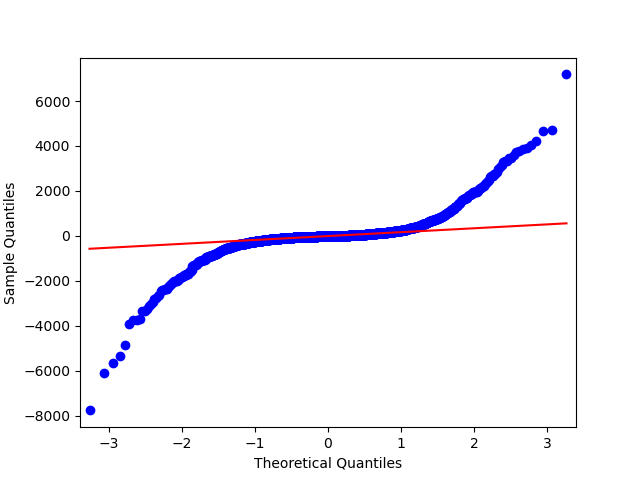
\includegraphics[width=6.0cm]{figures/btc_arima_residual.png}
			}
			\subfigure[Bitcoin Residual Q-Q Plot]{
				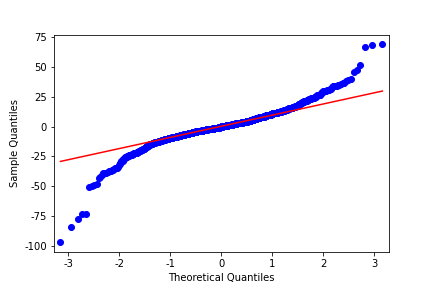
\includegraphics[width=6.0cm]{figures/gold_arima_residule.png}
			}
		\end{center}
			\caption{Residual Q-Q Plot for Gold and Bitcoin}
		\label{fig:qq_plot}
	\end{figure}

	We can see in Figure \ref{fig:qq_plot} that the scatters appears to be around a straight line, which indicates our parameters are good enough to predict the future.
	
	\item \textbf{DW Test}
	DW test is commonly used for test whether autocorrelation presents in the residuals from a regression analysis. The DW statistics has a null hypothesis
	
$$
	H_0 \ : \ \rho = 0	
$$
	And the test statistic is
	
	\begin{equation}\label{eqn:d}
		d \ = \ \frac{\Sigma_{t=2}^T(e_t-e_{t-1})^2}{\Sigma_{t=1}^T e_t^2}
	\end{equation}

	We calculate $d$ in equation \ref{eqn:d}, which is the approximation of $2(1-\hat{\rho})$, where $\hat{\rho}$ is the sample autocorrelation of the residuals. So $d=2$ indicates no autocorrelation. In our case, we calculate the values in by equation \ref{eqn:d}, and find
	$$
	d \ = \ 2.0179203733750732
	$$
	which is very close to 2, indicating very low autocorrelation. 
\end{enumerate}


\subsubsection{Predict the Change Using \Predictor}


\subsection{Trade Decision}

\subsubsection{Rating Gold and Bitcoin}

Based on the closing price every day, we first calculates the required normalized factors using including the change today, and the average change of 15 days and the bias, for both bitcoin and gold. Then our model predict the price the next day with ARIMA model.
	
Then, we calculate the indicators with the formula below for bitcoin and gold. 
	
	
\begin{align*}
Trend \ indicator &= TI = 0.7 \times 30 \ day's \ average change \ + \ 0.3 \times 20 \ day's \ average \ bias \\
Risk \ indicator &= RI = 0.4 \times Normalized \ 15 \ day's \ average \ change + 0.6 \times bias
\end{align*}
	
Then we compose $TI$ and $RI$ linearly with ratios chosen according to Markowiz's asset portfolio model and then normalize it to get our main factor ($MF$) for bitcoin and gold. 
	
We set following thresholds for selling or buying bitcoin and gold in Table \ref{table:threshold}.
	
\begin{table}[H]
		\renewcommand{\arraystretch}{1.5}
		\caption{Trading Thresholds.}
		\label{table:threshold}
		\begin{center}
			{\footnotesize
				\begin{tabular}{c c c}
					\toprule
					{ } & {Bitcoin} & {Gold} \\
					\midrule
					Buy($BS$) & 0.775 & 0.57 \\
					Sell($SS$) & 0.55 & 0.3 \\
					\bottomrule
			\end{tabular}}
		\end{center}	
\end{table}
	
Then, we trade bitcoin and gold subject to the following rules.
	
\begin{center}
		\begin{tabular}{ |c|c|c|c| } 
			\hline
			& $MF_{bitcoin} > BS_{bitcoin}$ & $Others$ & $MF_{bitcoin} < SS_{bitcoin}$ \\ 
			\hline
			$MF_{gold} > BS_{gold}$ & \textbf{\textit{Further Judgment Required}}  & Buy gold & Sell bitcoin and buy gold  \\ 
			\hline
			Others & Buy bitcoin & Do nothing & Sell bitcoin \\
			\hline
			$MF_{gold} < SS_{gold}$ & Sell gold and buy bitcoin & Sell gold & Sell both \\ 
			\hline
		\end{tabular}
\end{center}
	
When further judgment is required, we come up with the following factor $F$ 
	
$$
F=2.5 \times (MF_{bitcoin}-BS_{bitcoin})-(MF_{gold}-BS_{gold})
$$
	
Then, our model recommend buying gold when $F<0$ and buying bitcoin when $F>0$.

\subsubsection{Position Management}



\begin{figure}[H]
	\centering{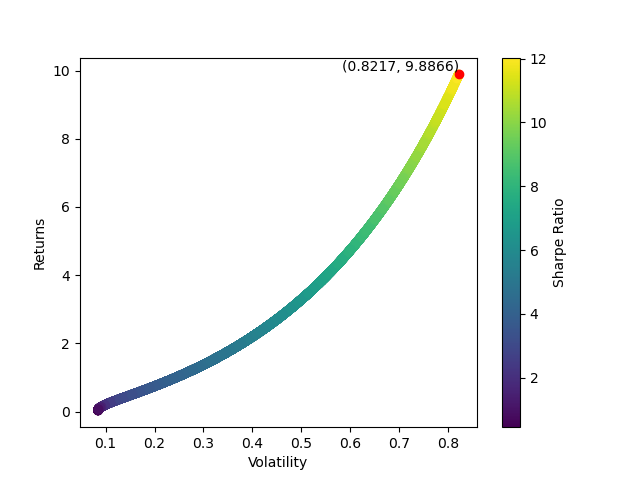
\includegraphics[width=8.0cm]{figures/markowiz_sim.png}}
	\caption{Application of Markowiz Model}
	\label{figure:markowiz}
\end{figure}



%%%%%%%%%%%%%%%%%
\section{Results and Solutions}
\label{Results_Solutions}

\begin{figure}[H]
	\centering{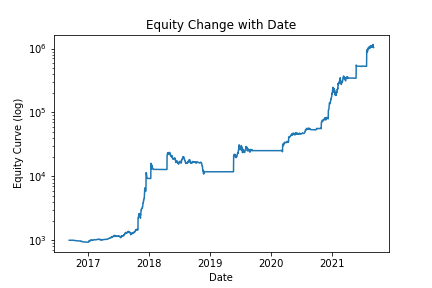
\includegraphics[width=8.0cm]{figures/equity_change.png}}
	\caption{Equity Change Result}
	\label{figure:equity_change}
\end{figure}

As is plotted in Figure \ref{figure:equity_change}, our equity change rises a lot with time going by. From the plot we can know the following facts.

\begin{itemize}
	\item \textbf{Our strategies work well to maximize income.} As is seen in the plot, the equity rises in the order of magnitude from $10^3$ to $10^6$, which is a considerable achievement.
	
	\item \textbf{Our strategies has a distinct feature that it has very low retracement.} As is seen in the plot, only there are only a few retracements, all of which have small value changes. It reveals that we have a good performance in dealing with risks.
\end{itemize}

The detailed performance data is shown in Table \ref{table:performance}. From the table we can have a quantitative view on the brilliant performance of our model.

\begin{table}[H]
	\renewcommand{\arraystretch}{1.5}
	\caption{Performance Data}
	\label{table:performance}
	\begin{center}
		{\footnotesize
			\begin{tabular}{c c }
				\toprule
				Performance Indicator & Measurement\\
				\midrule
				Accumulated Equity & $1.03743 \times 10^6$ \\
				Annualized Return & 1469.58\% \\
				Maximum Retracement & -53.90\% \\
				Annualized Return/Retracement Ratio & 27.77 \\
				Sharpe Ratio & 1.1358 \\
				\bottomrule
		\end{tabular}}
	\end{center}	
\end{table}



%%%%%%%%%%%%%%%%%
\section{Sensitivity Analysis}
\label{SensitivityAnalysis}

For each transaction, a commission is charged. The commission can also have an impact on our model. We tested our model with different commissions and found that the level of commission does not significantly affect our model.

 \begin{figure}[H]
	\centering{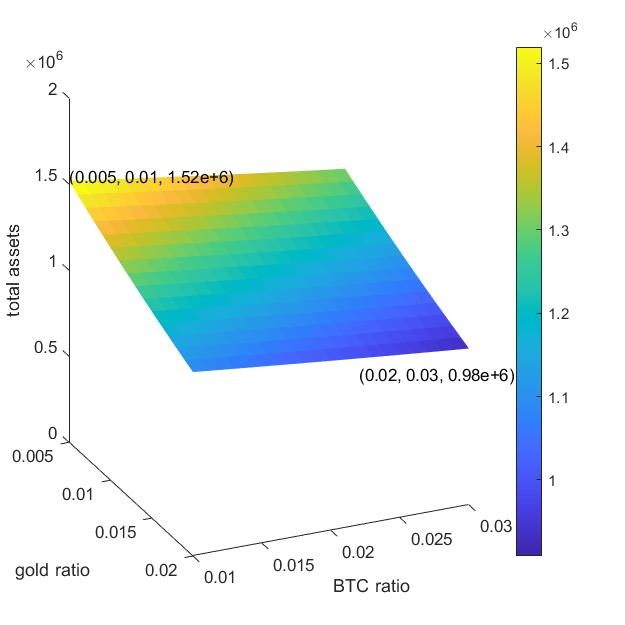
\includegraphics[width=8.0cm]{figures/sensitive_test.jpg}}
	\caption{Equity Change with Commissions}
	\label{figure:sensitive_test}
\end{figure}

By changing commissions and recalculating the total assets we get, we plot Figure \ref{figure:sensitive_test}, from which we can draw the following conclusions

\begin{enumerate}
	\item Commissions may influence the equity change in the end, but the range is considered small, which reveals great stability of our model.
	
	\item From the figure we plot, we find that commissions for bitcoins have a stronger impact on the income. It is because to reach higher income, we hold more bitcoins so that when commissions go higher, we are charged much more.
	
	\item The given commissions is higher than the commissions in the real world, 0.02\% for bitcoin and 0.05\% for gold. When choosing the thresholds for trading, we can choose more suitable parameters and trade in lower frequencies to reduce frictional costs.
\end{enumerate}

%%%%%%%%%%%%%%%%%
\section{Strength and Weakness}
\label{Strength_Weakness}


\subsection{Strength}

The models have the following strengths:

\begin{itemize}
\item \textbf{Our model yields considerable income}

\item \textbf{Our model do not involve artificial neural network, which saves computational resources.}

\item \textbf{Our model build up a good system to assess a financial asset.}

\item \textbf{Our model can be generalized to all problems in trading.}

\end{itemize}


\subsection{Weakness}

Though our model performs well, the models have following weaknesses:

\begin{itemize}
\item \textbf{We do not consider factors other than prices.}

\item \textbf{The choice of our model's parameters relies on experience and grid search.}
\end{itemize}


%%%%%%%%%%%%%%%%%
\section{Conclusions}
\label{Conclusions}

In this paper, we build a \Predictor based predictor to enhance the income of trading cash, gold, and bitcoins. First, we preprocess the data and fill the missing values. Then, we finish the feature engineering by finite difference and feature store to boost the machine learning effect. After that, we use a RNN-based \Predictor to predict the price. Finally, we reach the optimality of our model by compare different trading strategies. Sensitive tests and evaluation are carried out. We measured our model by annualized return, retracement and sharp rate. The influence of commissions are experimented to test the sensitivity. Our model yields satisfying results.




%%%%%%%%%%%%%%%%%
\newpage
\begin{thebibliography}{00}

%% \bibitem{label}
%% Text of bibliographic item

\bibitem{Du2021}
Lin Hongmei,Du Jinyan,Zhang Shaodong. Sharpe ratio: estimation method, applicability and empirical analysis[J]. Journal of Statistics,2021,2(06):73-88.DOI:10.19820/j.cnki.issn2096-7411.2021.06.006.

\bibitem{Sun2020}
Sun, Lipo. An empirical study of Makowitz's portfolio theory based on Python[J]. Times Finance,2020(25):46-47+50.

\bibitem{Pierre2020}
Pierre Rostan,Alexandra Rostan,Mohammad Nurunnabi. Options trading strategy based on ARIMA forecasting[J]. PSU Research Review,2020.


\bibitem{Marcos2018}
Marcos Lopez dai Prado, \textit{Advances in Financial Machine} Learning[M]:75-82. ISBN 978-1119482086

\bibitem{Li2017}
Li F. Modelling the stock market using a multi-scale approach[D]. University of Leicester, 2017.

\bibitem{Lin2016}
Lin Xiaoming, A preliminary exploration of Huatai's multi-factor model system [R], Huatai Securities, 2016.

\bibitem{Pang2005}
Marling H, Emanuelsson S. The Markowitz Portfolio Theory[J]. November, 2012, 25: 2012.


\end{thebibliography}
\addcontentsline{toc}{section}{References}


\addtocounter{page}{-1}
\thispagestyle{empty}

%%%%%%%%%%%%%%%%%
\newpage
\addtocounter{page}{-1}
\thispagestyle{empty}

{\centering\section*{Memorandum to the Trader}}

Considering the intensely changing financial markets and the difficulty of handling your portfolio, using an appropriate model to make predictions and strategies to trade are of vital importance to improve income. It is a great honor for us to develop the model for you to buy, hold and sell your assets. Here is our model based on \textbf{\Predictor} and strategies for you to trade your assets effectively.  
	
\begin{enumerate}
	\item Our model calculates the required normalized factors using the closing price every day,including the change today, the average change of 15 days and the bias, for both bitcoin and gold. Then our model predict the price the next day with ARIMA model.
	 
	\item Based on the calculated values and our research, we calculate the indicators with the formula below for bitcoin and gold. 
	

\begin{align*}
	Trend \ indicator &= TI = 0.7 \times 30 \ day's \ average change \ + \ 0.3 \times 20 \ day's \ average \ bias \\
	Risk \ indicator &= RI = 0.4 \times Normalized \ 15 \ day's \ average \ change + 0.6 \times bias
\end{align*}
	
	Then we compose $TI$ and $RI$ linearly with ratios chosen according to Markowiz's asset portfolio model and then normalize it to get our main factor ($MF$) for bitcoin and gold. 
	
	\item We set following thresholds for selling or buying bitcoin and gold in Table \ref{table:memo_threshold}.
	
	\begin{table}[H]
		\renewcommand{\arraystretch}{1.5}
		\caption{Trading Thresholds.}
		\label{table:memo_threshold}
		\begin{center}
			{\footnotesize
				\begin{tabular}{c c c}
					\toprule
					{ } & {Bitcoin} & {Gold} \\
					\midrule
					Buy($BS$) & 0.775 & 0.57 \\
					Sell($SS$) & 0.55 & 0.3 \\
					\bottomrule
			\end{tabular}}
		\end{center}	
	\end{table}

	Our model trades bitcoin and gold subject to the following rules.
	
	\begin{center}
		\begin{tabular}{ |c|c|c|c| } 
			\hline
			 & $MF_{bitcoin} > BS_{bitcoin}$ & $Others$ & $MF_{bitcoin} < SS_{bitcoin}$ \\ 
			\hline
			$MF_{gold} > BS_{gold}$ & \textbf{\textit{Further Judgment Required}}  & Buy gold & Sell bitcoin and buy gold  \\ 
			\hline
			Others & Buy bitcoin & Do nothing & Sell bitcoin \\
			\hline
			$MF_{gold} < SS_{gold}$ & Sell gold and buy bitcoin & Sell gold & Sell both \\ 
			\hline
		\end{tabular}
	\end{center}

	When further judgment is required, we come up with the following factor $F$ 
	
	$$
	F=2.5 \times (MF_{bitcoin}-BS_{bitcoin})-(MF_{gold}-BS_{gold})
	$$
	
	Then, our model recommend buying gold when $F<0$ and buying bitcoin when $F>0$.
\end{enumerate}

With above strategies, our model achieve great income. The performance of our model is as follows

	\begin{table}[H]
	\renewcommand{\arraystretch}{1.5}
	\caption{Performance}
	\label{table:memo_performance}
	\begin{center}
		{\footnotesize
			\begin{tabular}{c c }
				\toprule
				Performance Indicator & Measurement\\
				\midrule
				Accumulated Equity & $1.03743 \times 10^6$ \\
				Annualized Return & 1469.58\% \\
				Maximum Retracement & -53.90\% \\
				Annualized Return/Retracement Ratio & 27.77 \\
				Sharpe Ratio & 1.1358 \\
				\bottomrule
		\end{tabular}}
	\end{center}	
\end{table}


We appreciate this opportunity to help you to build up a trading strategy for cash, gold and bitcoins, and we firmly believe that our model can be utilized in your tradings to maximize your income. Feel free to contact us for further information on the proposal.

Sincerely yours

\textit{MCM 2022 Team}



\end{spacing}


%%%%%%%%%%%%%%%%%
\newpage
%% The Appendices part is started with the command \appendix;
%% appendix sections are then done as normal sections
\appendix
\addtocounter{page}{-1}
\thispagestyle{empty}

\section*{Appendix: Figures and Tables}
\label{sec:AppendixFT}

\begin{figure}[H]
	\centering{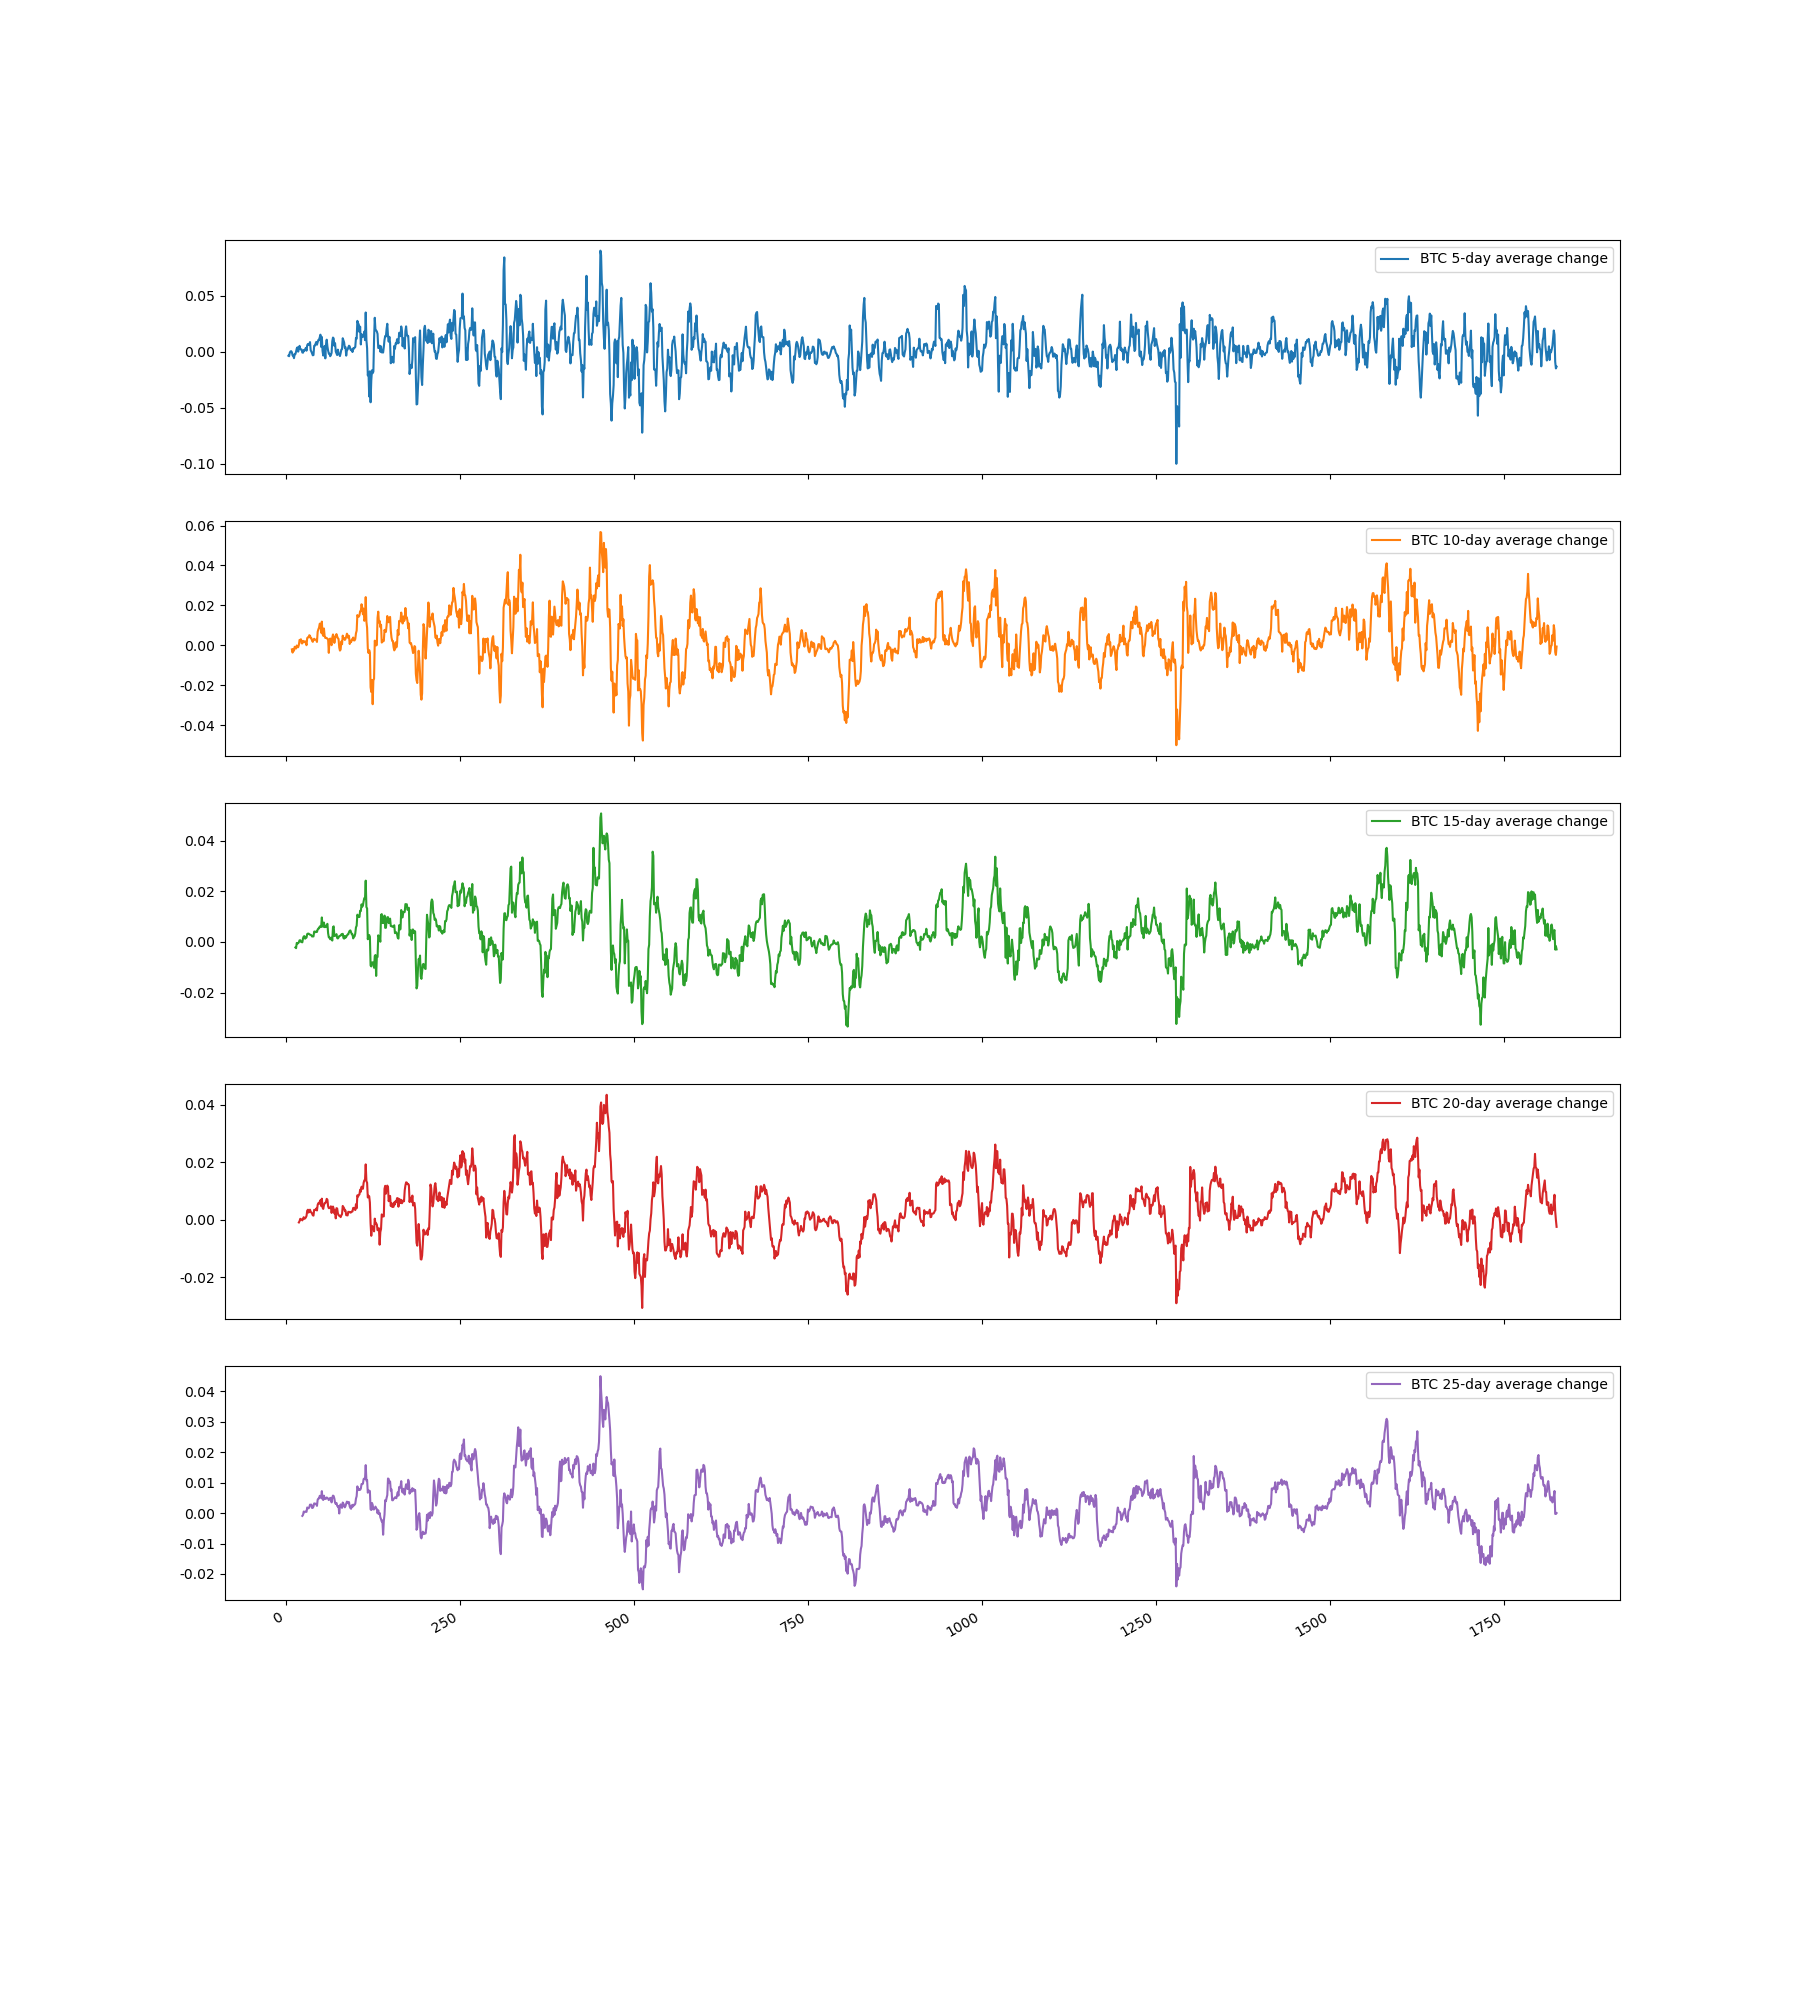
\includegraphics[width=17.0cm]{figures/bitcoin_ac.png}}
	\caption{ Average Change in 5,10,15,20,25 days for bitcoin}
	\label{figure:bitcoin_ac}
\end{figure}

\begin{figure}[H]
	\centering{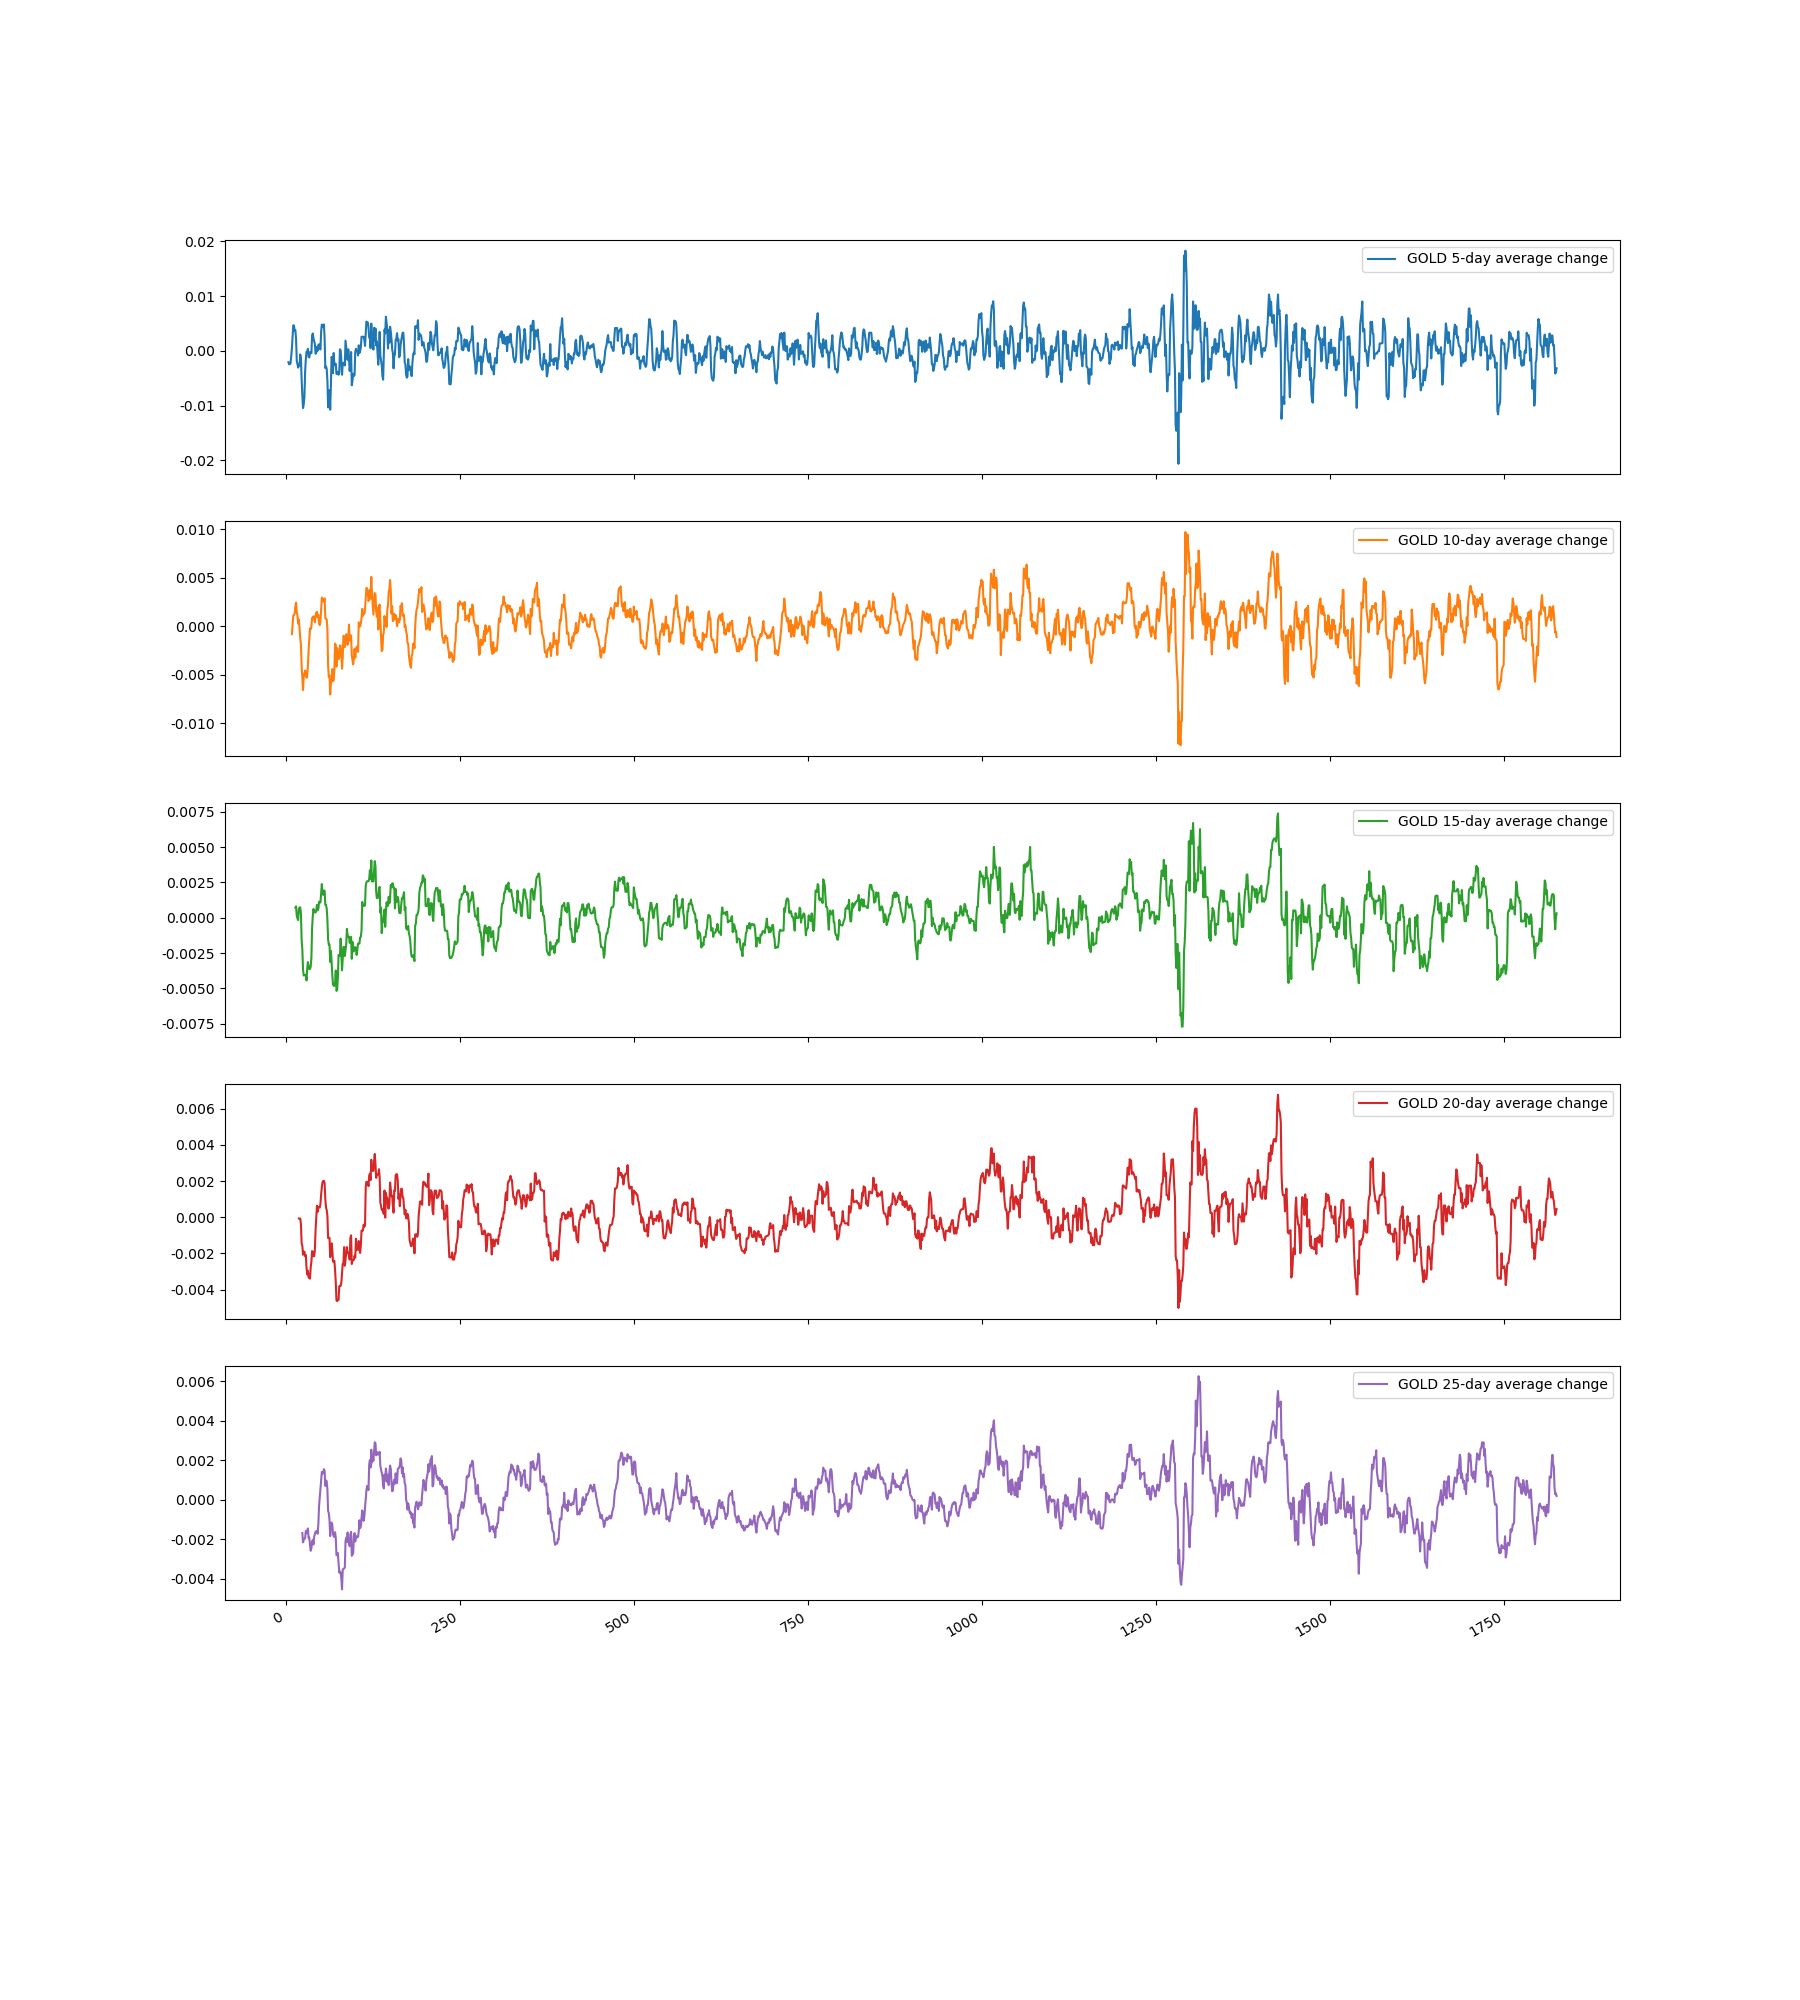
\includegraphics[width=17.0cm]{figures/gold_ac.png}}
	\caption{ Average Change in 5,10,15,20,25 days for gold }
	\label{figure:gold_ac}
\end{figure}


\end{document}


%% End of template
